%% ============================================================================
%%  Supporting Information for main.tex
%%  ---------------------------------------------------------------------------
%%  Compile with XeLaTeX (same as main.tex). Tables and figures are written by
%%  the R pipeline (R/tab1_model_selection.R, R/fig_supp.R,
%%  R/figS7_predictions.R) and pulled in directly, so they never drift from the
%%  fitted models. main.tex refers to them by number (Supplementary Fig. S1,
%%  ...), so keep the order here matched to the order of citation there.
%% ============================================================================

\documentclass[11pt]{article}

% ---- Encoding & page geometry ----------------------------------------------
\usepackage[utf8]{inputenc}
\usepackage[margin=1.25in]{geometry}

% ---- Colour & links --------------------------------------------------------
\usepackage[dvipsnames]{xcolor}
\definecolor{niceblue}{HTML}{236899}
\usepackage{hyperref}
\hypersetup{
    colorlinks=true,
    linkcolor=black,
    urlcolor=niceblue,
    citecolor=niceblue
}

% ---- Figures, floats, tables -----------------------------------------------
\usepackage{graphicx}
\usepackage{float}
\usepackage{placeins}     % \FloatBarrier
\usepackage{booktabs}     % \toprule \midrule \bottomrule
\usepackage{setspace}
\graphicspath{{../output/figs/supp/}}

% ---- Fonts (requires XeLaTeX/LuaLaTeX) -------------------------------------
\usepackage{fontspec}
\setmainfont{Libertinus Serif}

% ---- Supplementary numbering: Table S1, Figure S1, ... ---------------------
\renewcommand{\thetable}{S\arabic{table}}
\renewcommand{\thefigure}{S\arabic{figure}}
\renewcommand{\theHtable}{S\arabic{table}}
\renewcommand{\theHfigure}{S\arabic{figure}}

\date{}

% ============================================================================
\begin{document}
\onehalfspacing

\begin{center}
\textbf{\large Supporting Information}\\[0.5em]
\textbf{Linking predicted seascape connectivity, environment and spatial structure to cockle distribution in a coastal fjord}\\[0.5em]
Federico Maioli, Ane Pastor Rollan, Pedro S. Freitas, Camille Saurel, Isabelle Johansson, Flemming Thorbjørn Hansen, Martin Lindegren
\end{center}

% ---- Tables ----------------------------------------------------------------
\begin{table}[ht]
\centering
\caption{AIC of the full Space + Environment + Connectivity model with each of the five connectivity metrics, ordered by $\Delta$AIC (the best model is shown in bold). All metrics are presence-weighted; all models include survey, year, the environmental predictors and a spatial random field.}
\label{tab:connectivity-metrics}
\begin{tabular}{lrr}
\toprule
Connectivity metric & AIC & $\Delta$AIC \\
\midrule
In-strength & \textbf{29634.6} & \textbf{0.0} \\
Eigenvector centrality & 29636.3 & 1.7 \\
Transitivity & 29638.0 & 3.4 \\
In-degree & 29638.2 & 3.6 \\
In-closeness & 29638.2 & 3.6 \\
\bottomrule
\end{tabular}
\end{table}

\FloatBarrier
\clearpage

% ---- Figures, numbered in the order they are cited in main.tex -------------
\begin{figure}[H]
    \centering
    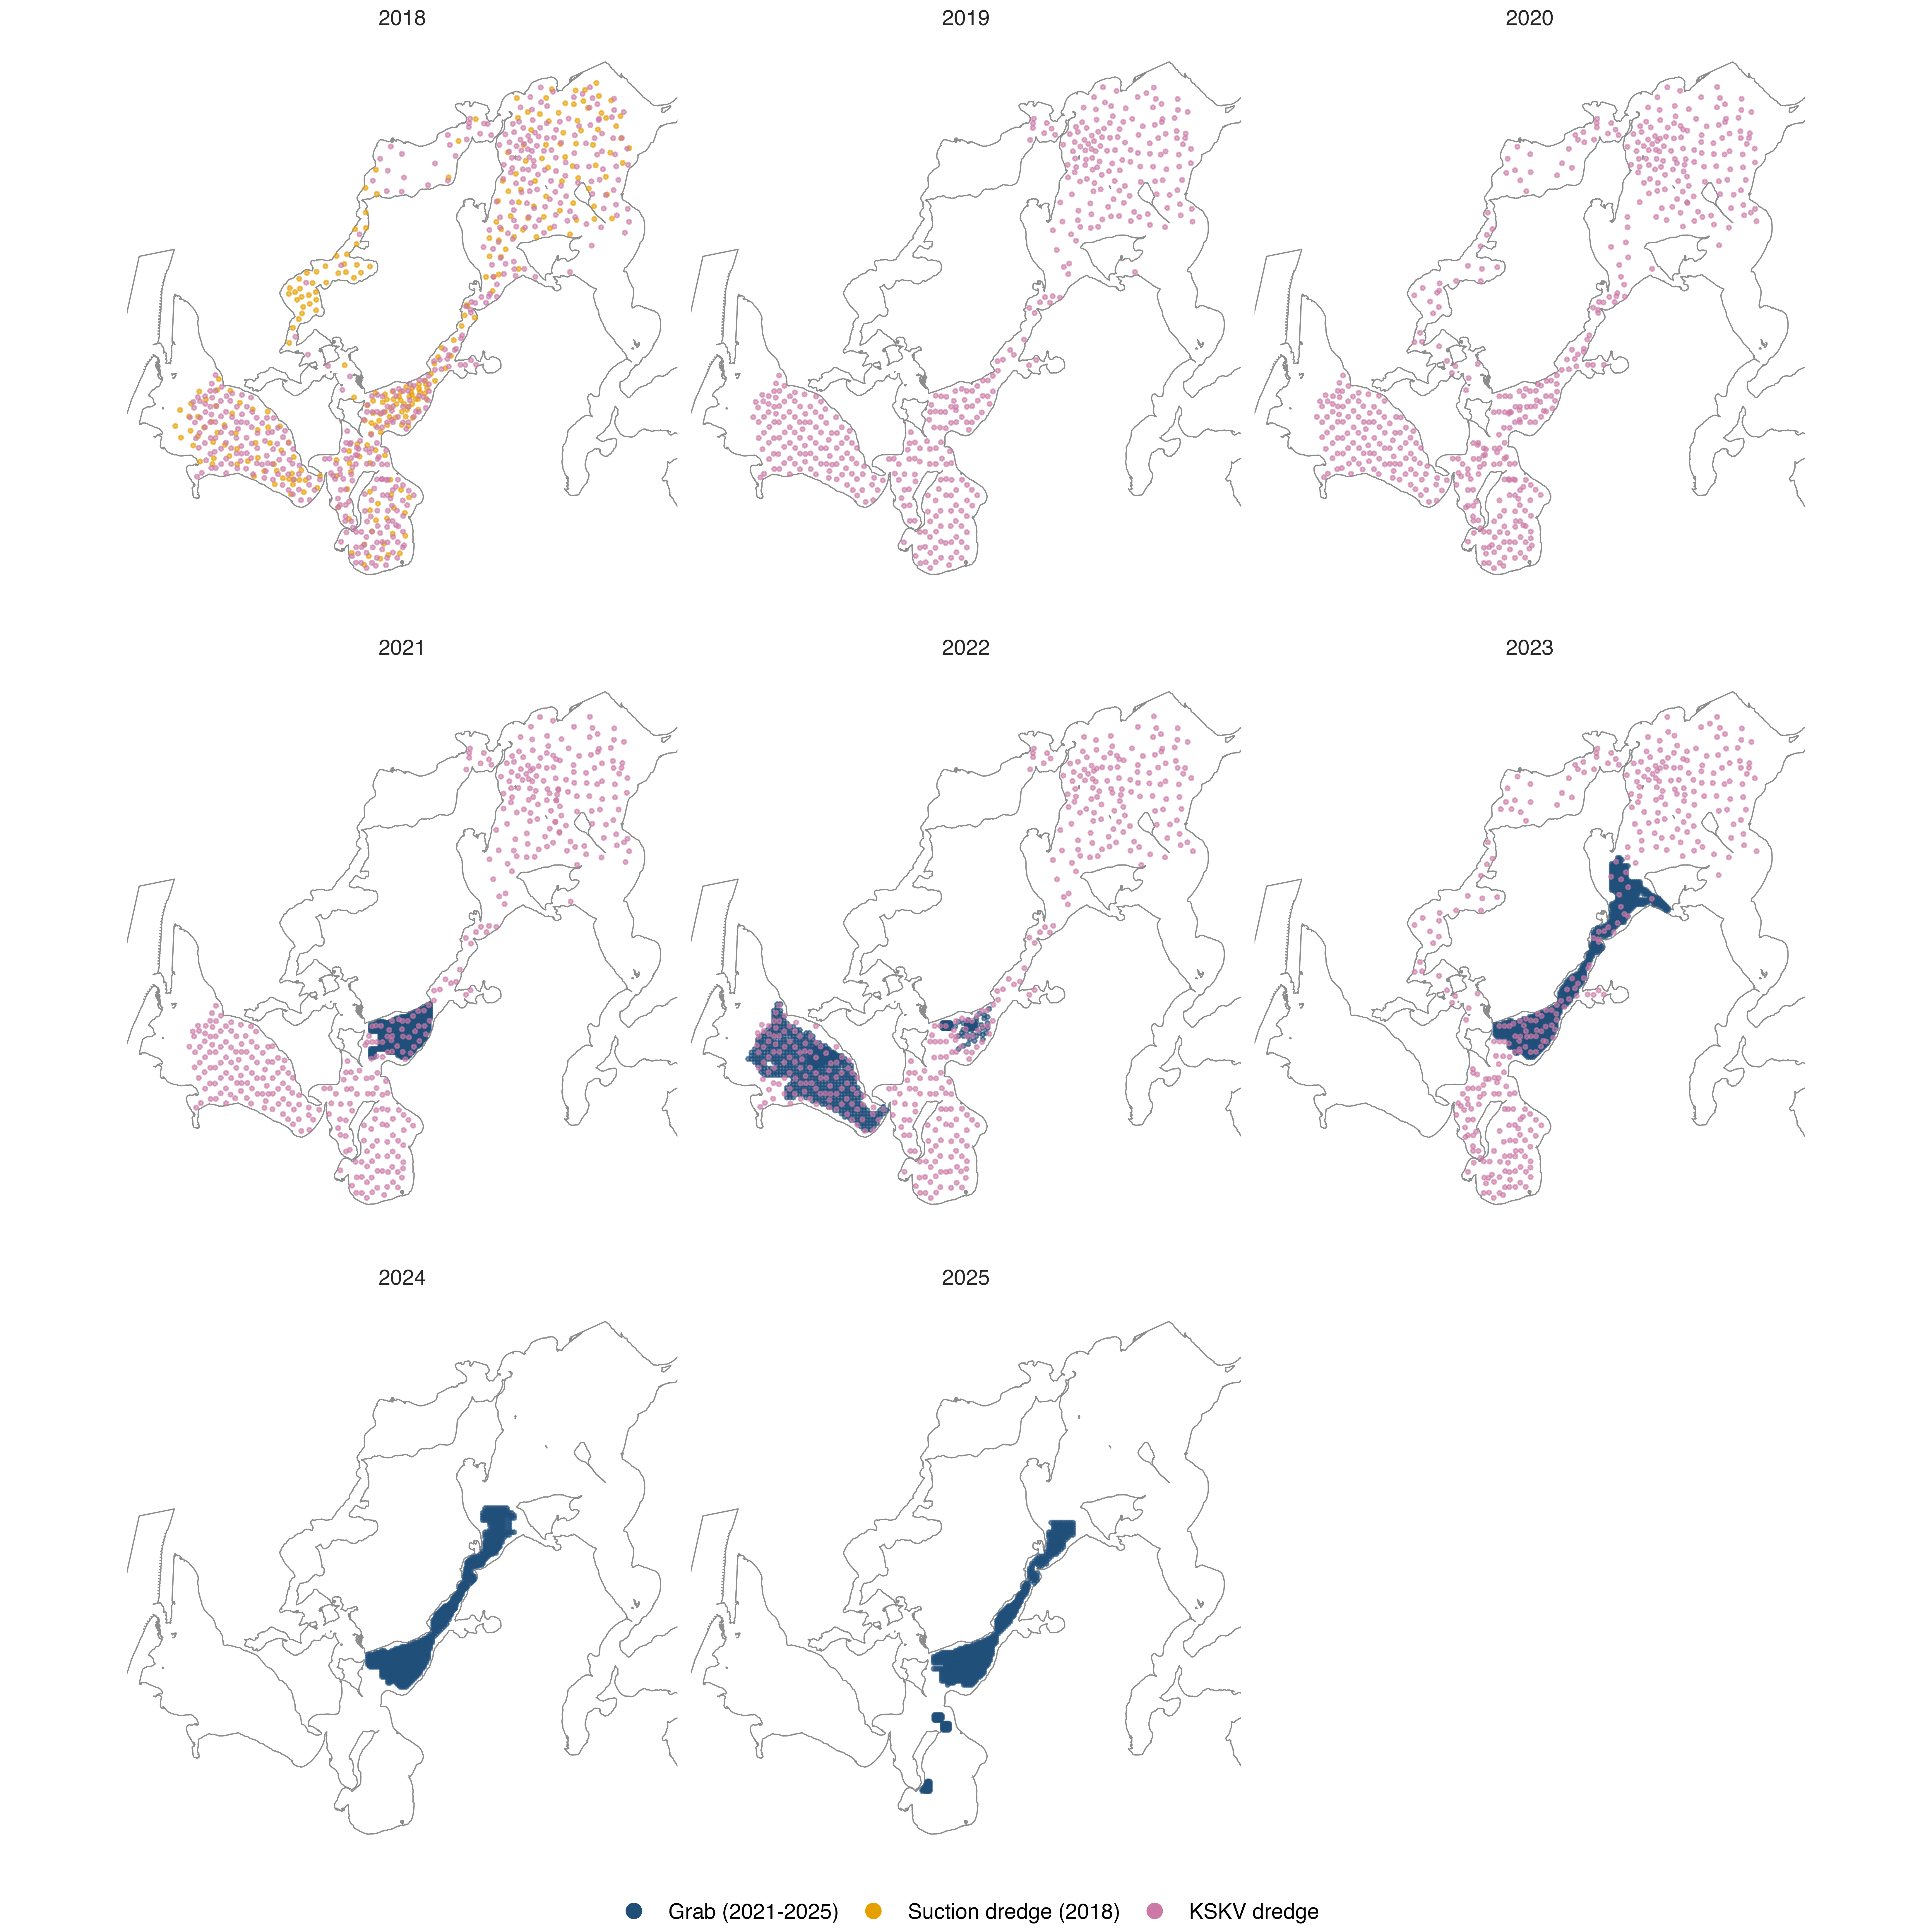
\includegraphics[width=0.85\textwidth]{figS1_survey_stations.png}
    \caption{Survey stations used in the models, by year and survey: the 2021--2025 grab surveys (including the high-resolution surveys of 2021--2022), the 2018 suction-dredge survey, and the 2018--2023 KSKV dredge surveys.}
    \label{fig:survey_stations}
\end{figure}
\clearpage

\begin{figure}[H]
    \centering
    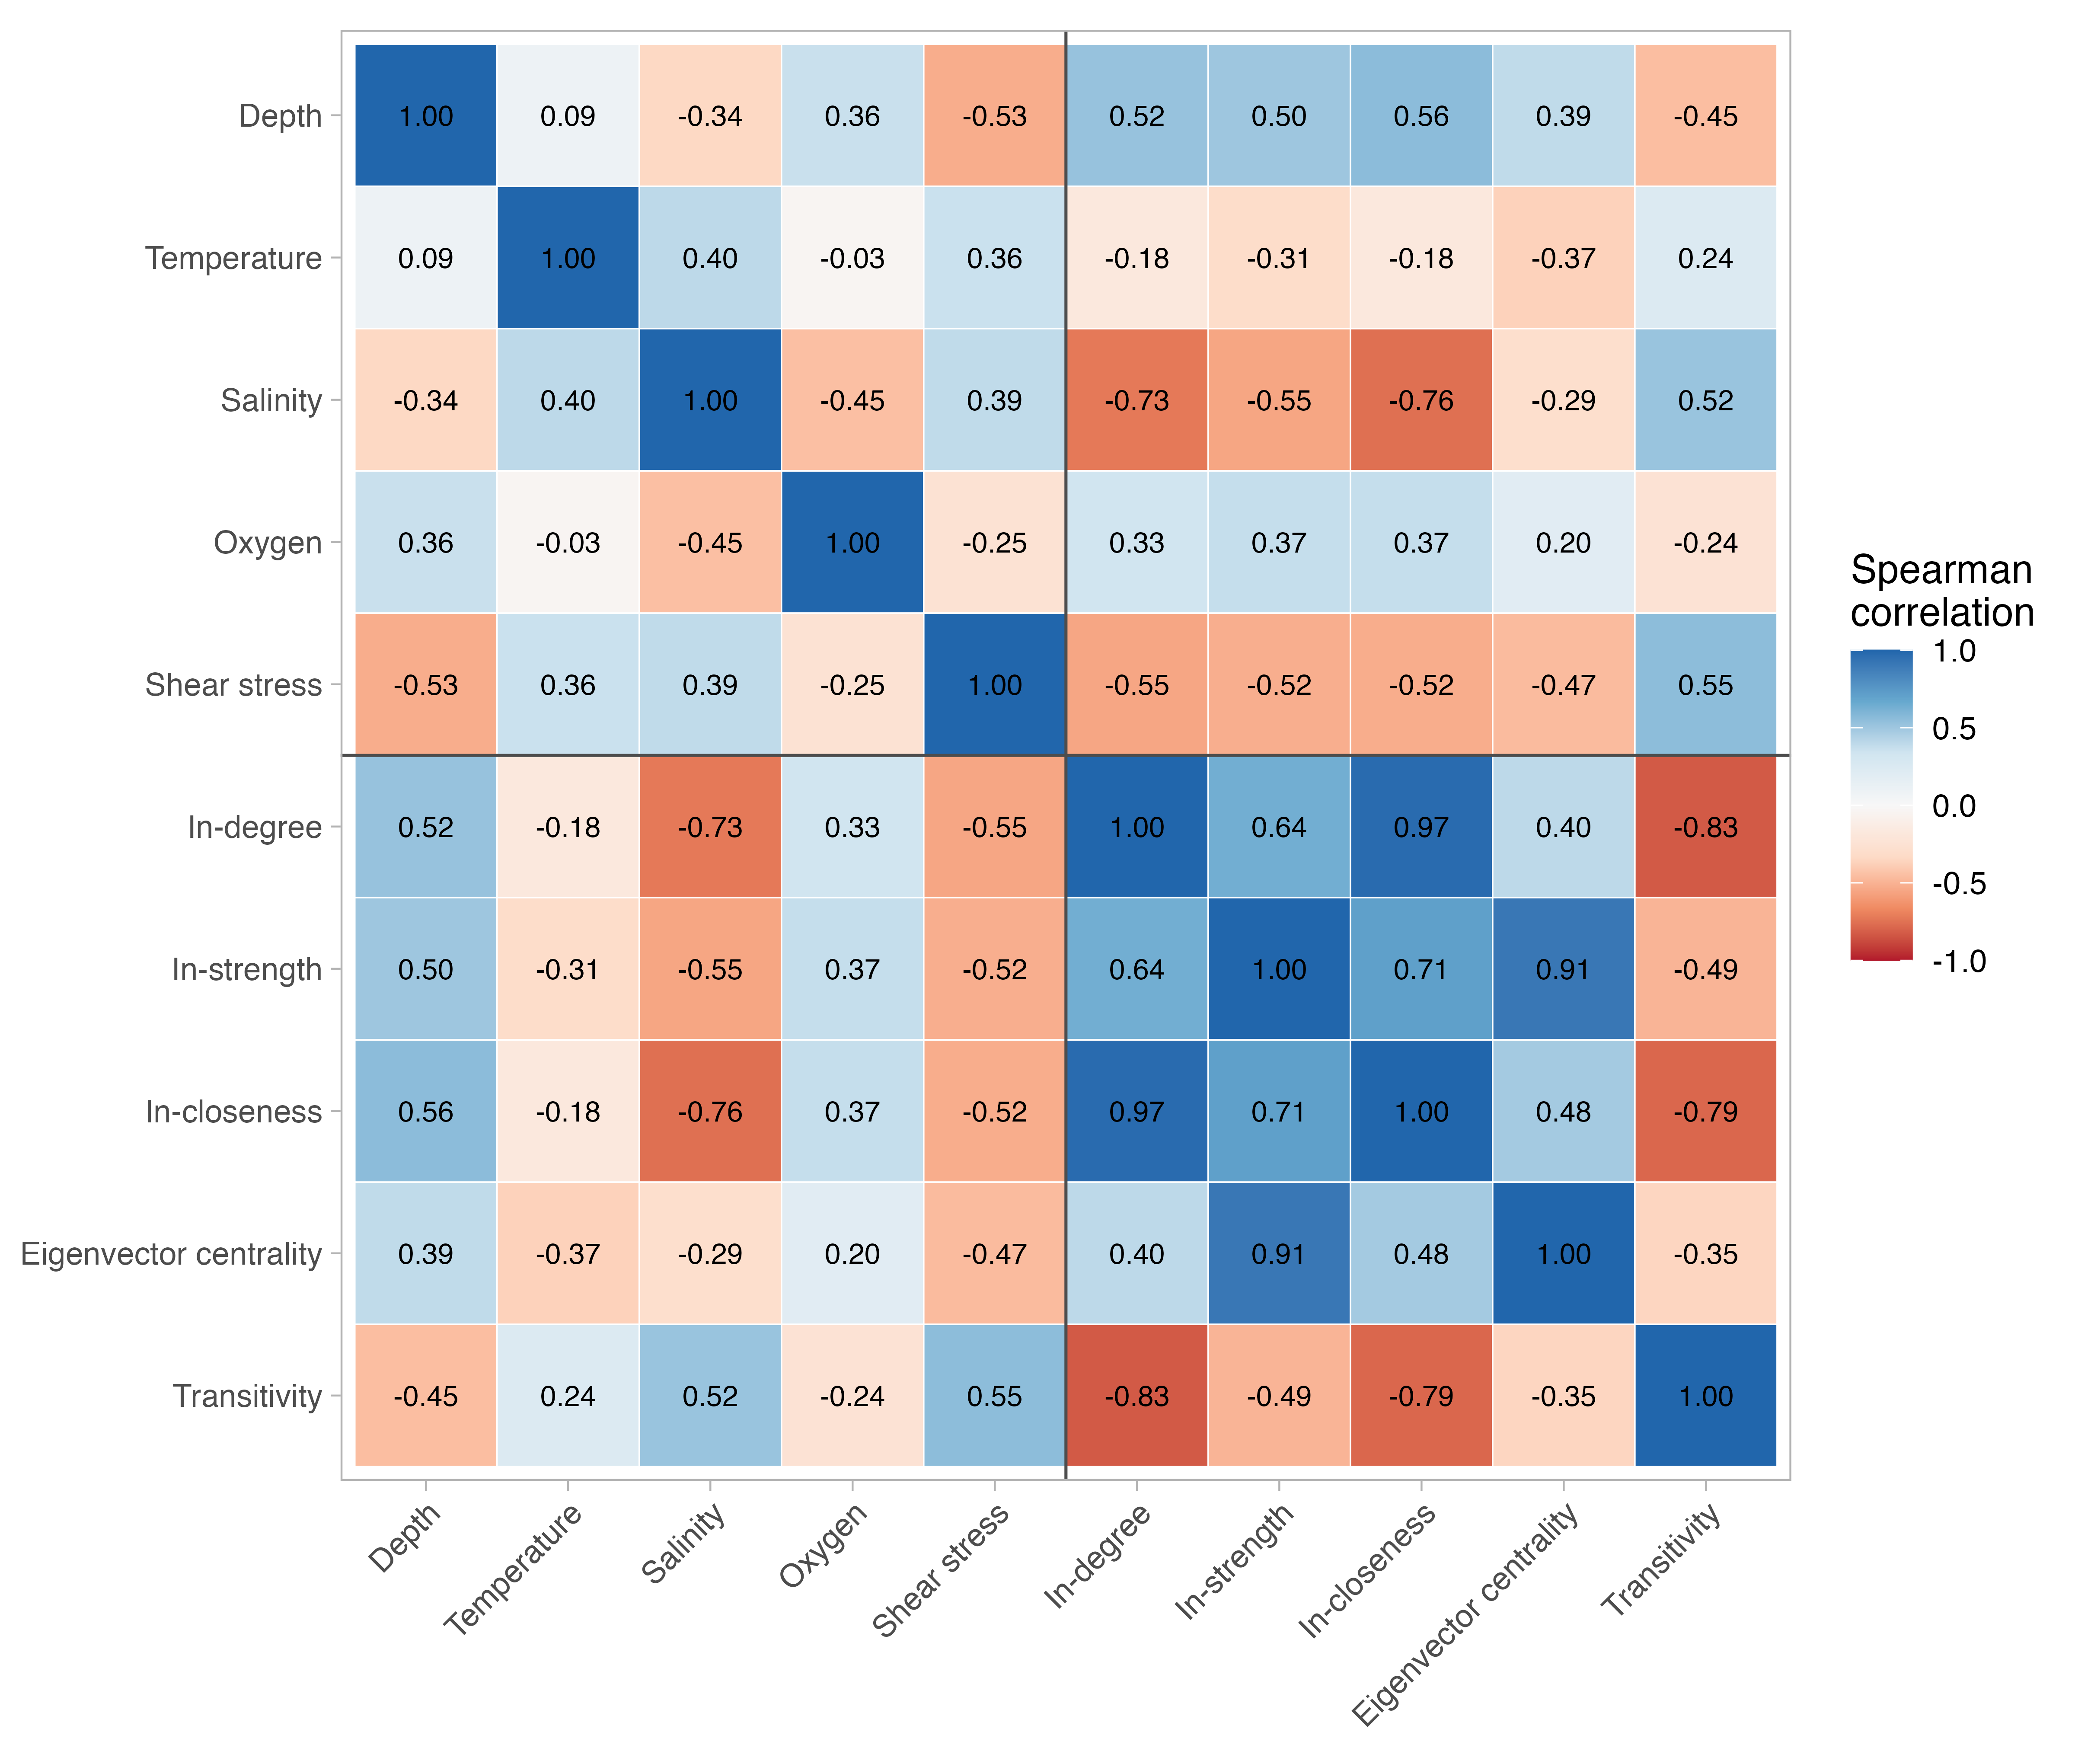
\includegraphics[width=0.8\textwidth]{figS2_correlation.png}
    \caption{Spearman correlation, at the survey stations, among the five environmental predictors and the five presence-weighted connectivity metrics. Lines separate environmental predictors from connectivity metrics.}
    \label{fig:correlation}
\end{figure}
\clearpage

\begin{figure}[H]
    \centering
    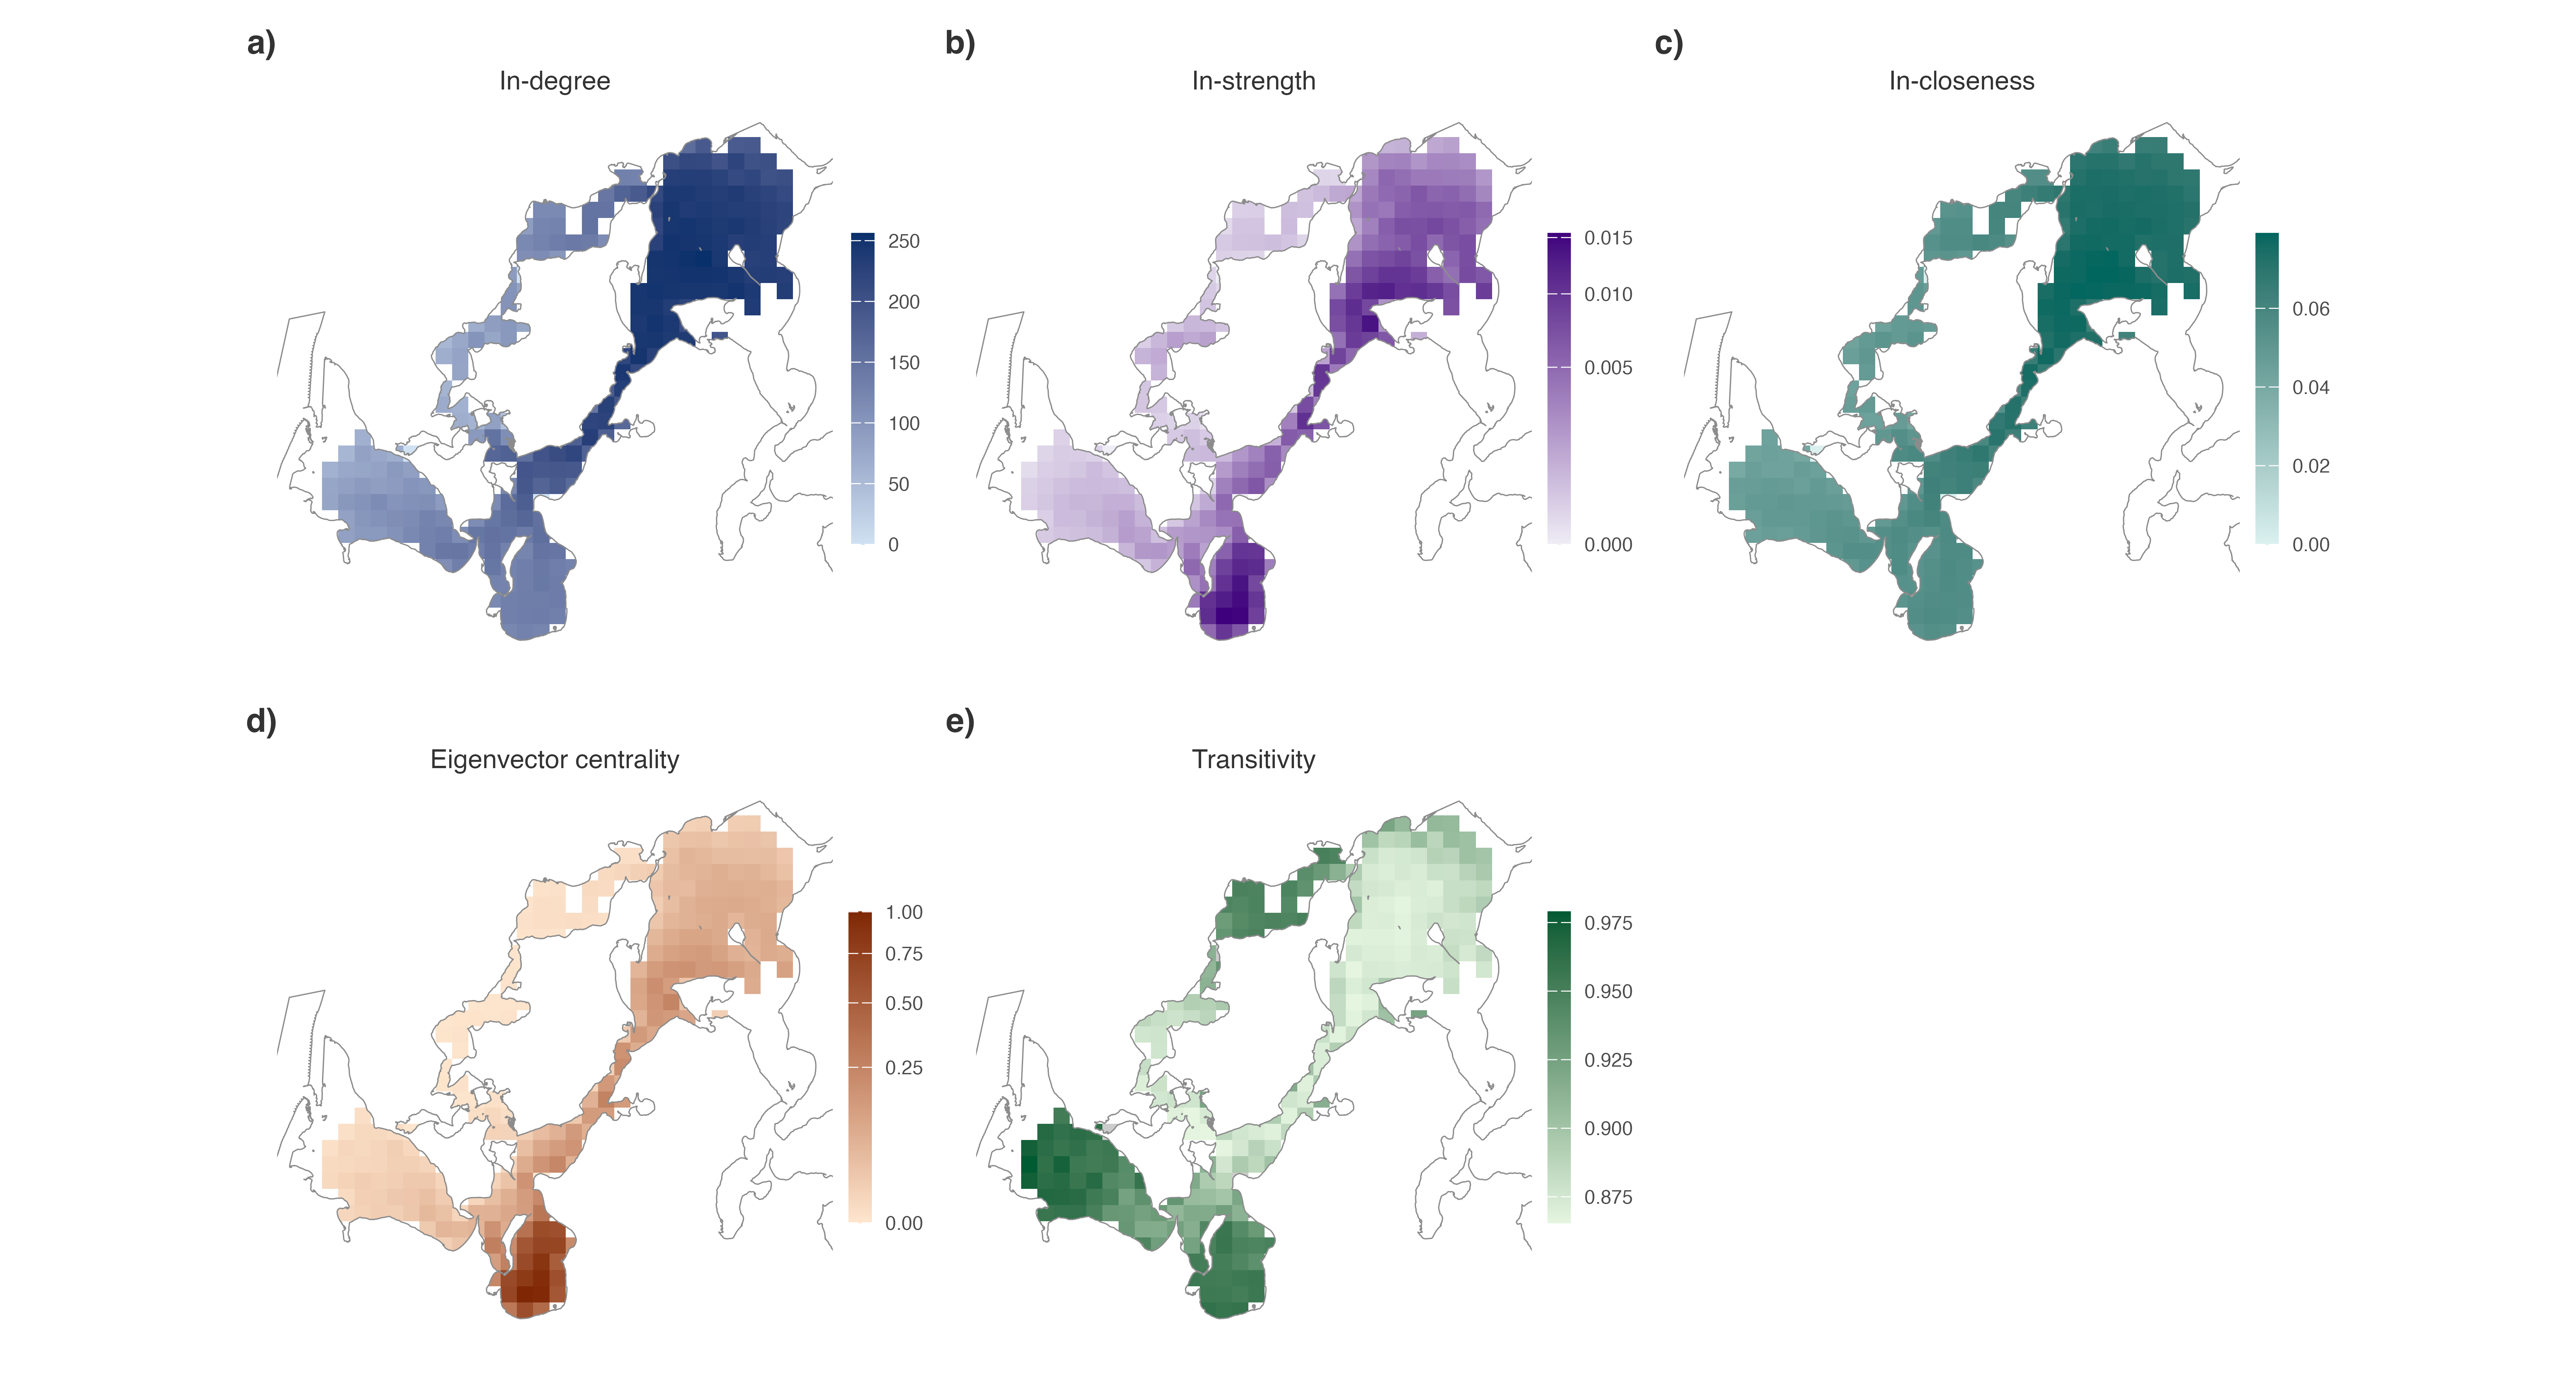
\includegraphics[width=0.95\textwidth]{figS3_connectivity_metrics.png}
    \caption{Presence-weighted connectivity metrics at the 2~$\times$~2~km grid cells containing at least one survey station: (a) in-degree, (b) in-strength, (c) in-closeness, (d) eigenvector centrality and (e) transitivity.}
    \label{fig:connectivity_maps}
\end{figure}
\clearpage

\begin{figure}[H]
    \centering
    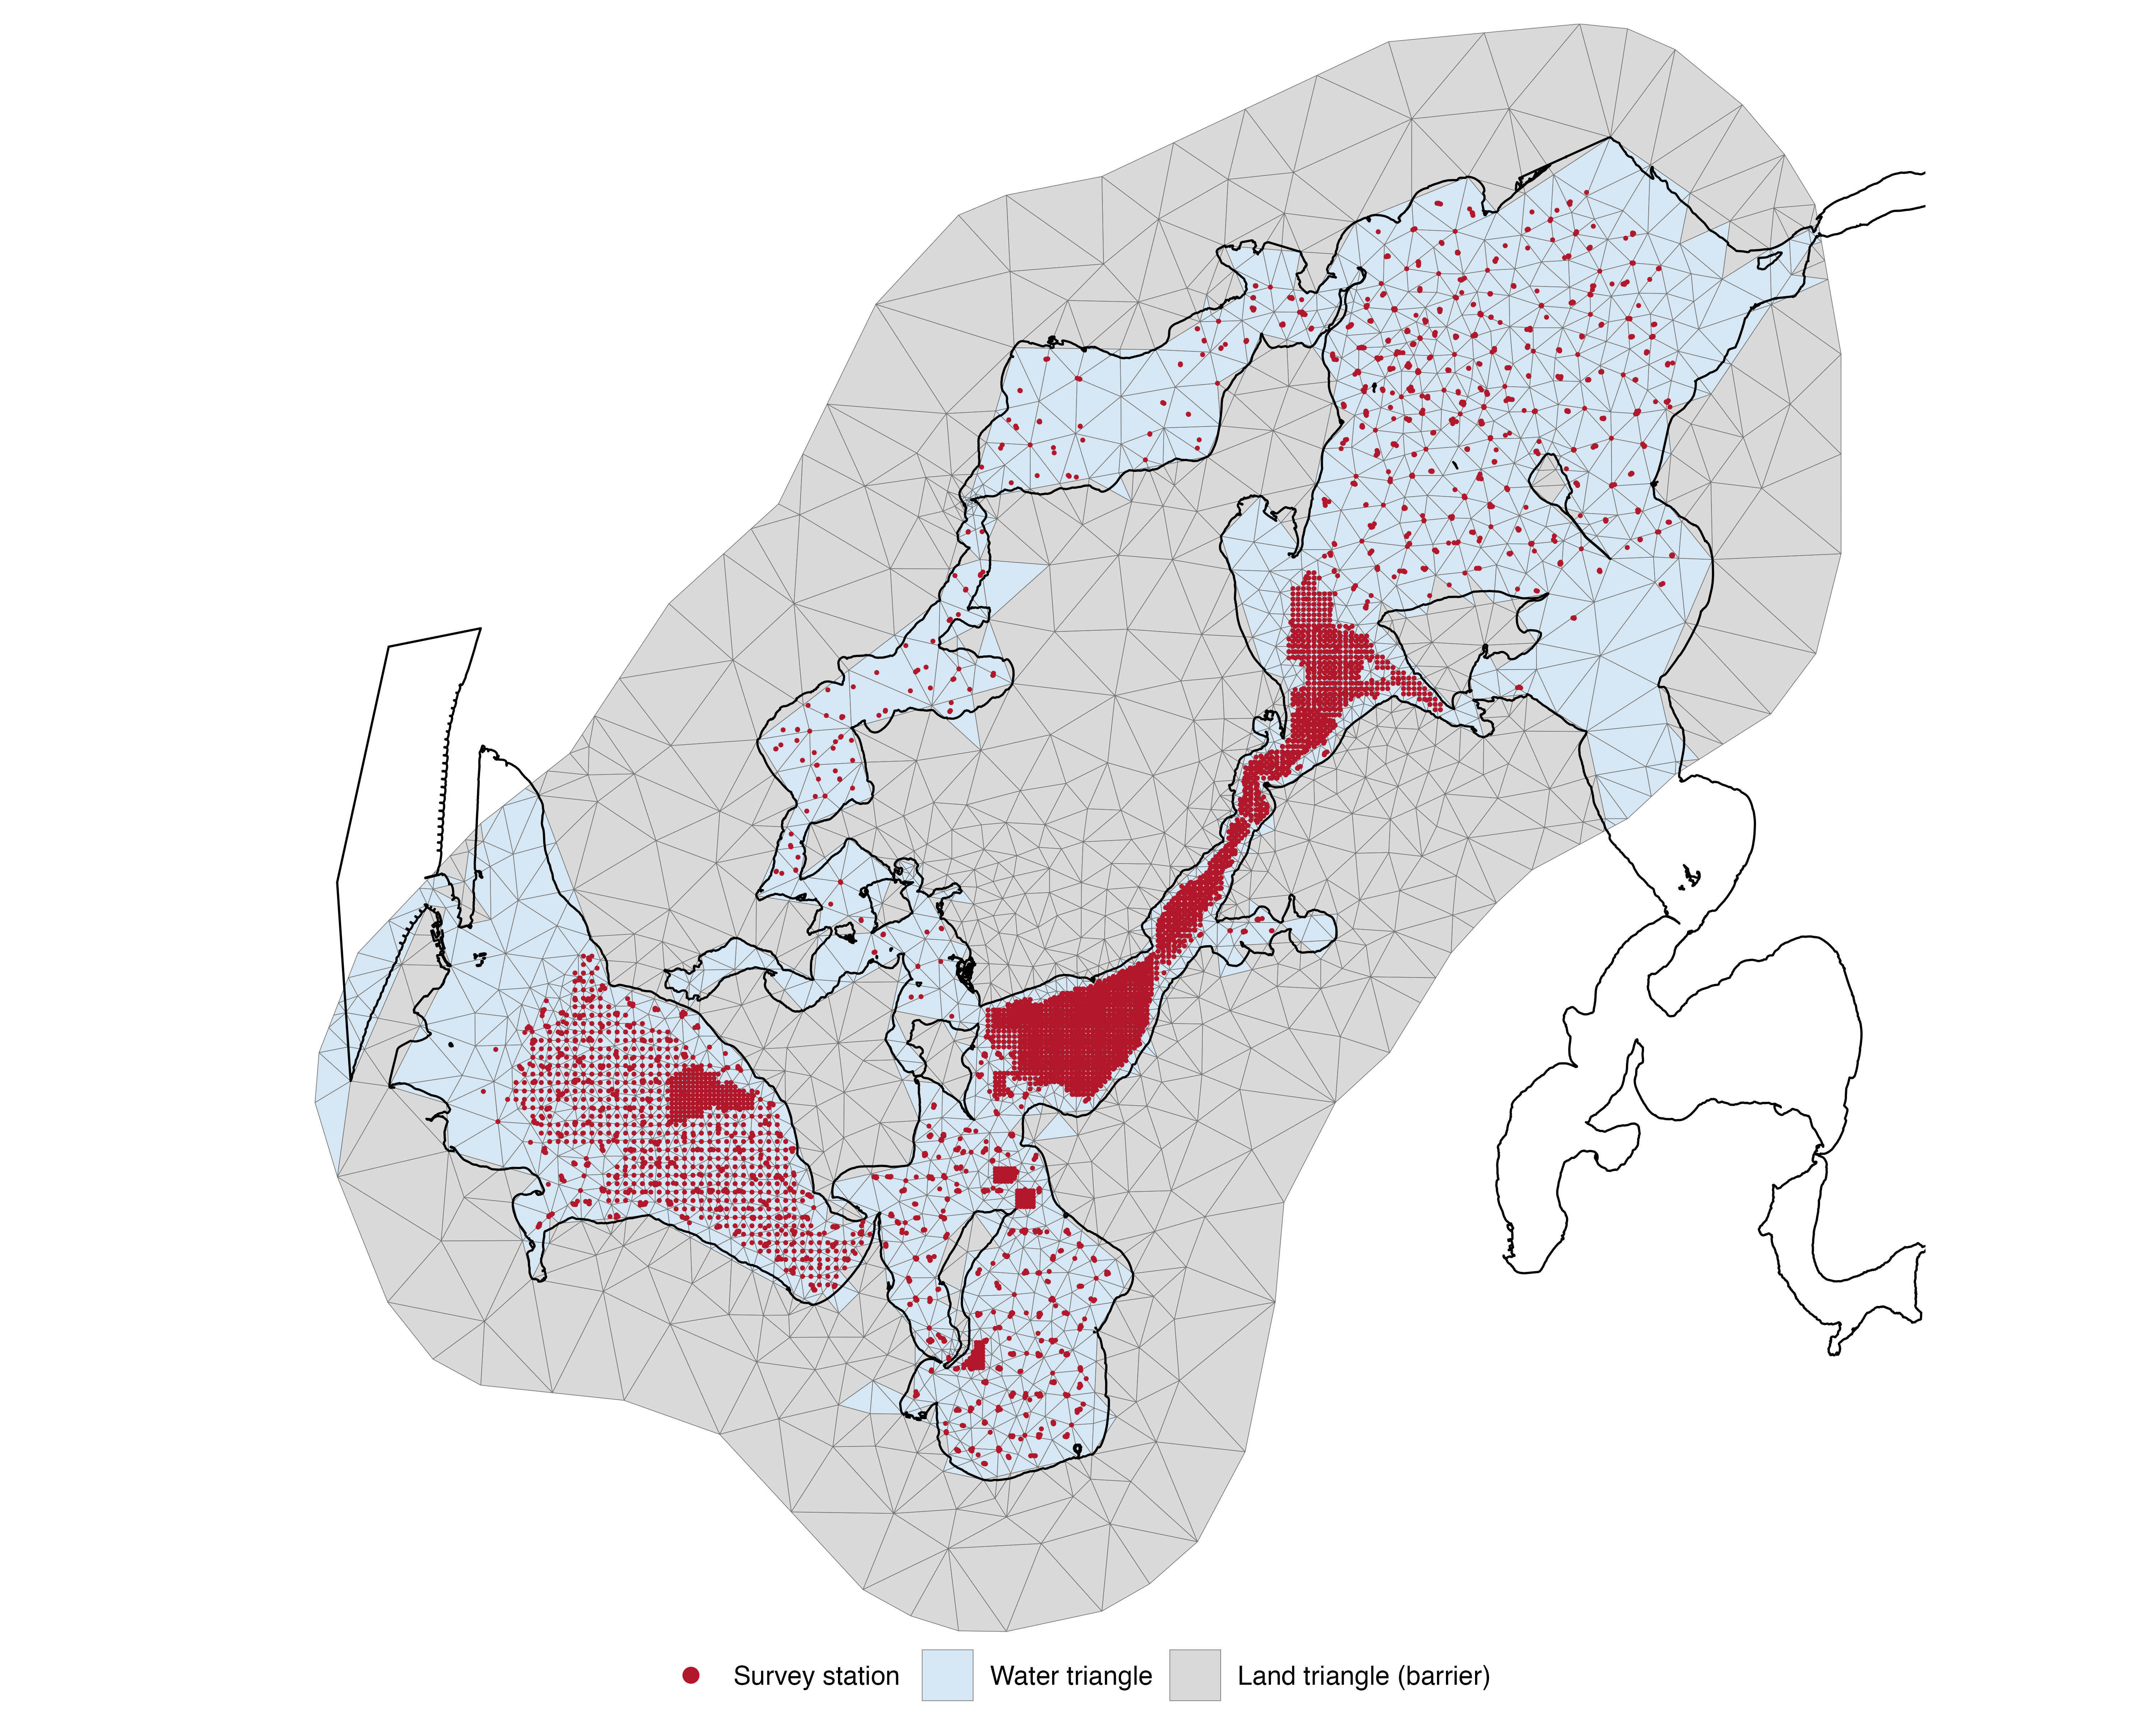
\includegraphics[width=0.95\textwidth]{figS4_mesh.png}
    \caption{Variable-resolution barrier mesh used for the spatial random field. Triangles on land (grey) form the barrier, in which the correlation range is 10\% of that in water (blue); red points are survey stations.}
    \label{fig:mesh}
\end{figure}
\clearpage

\begin{figure}[H]
    \centering
    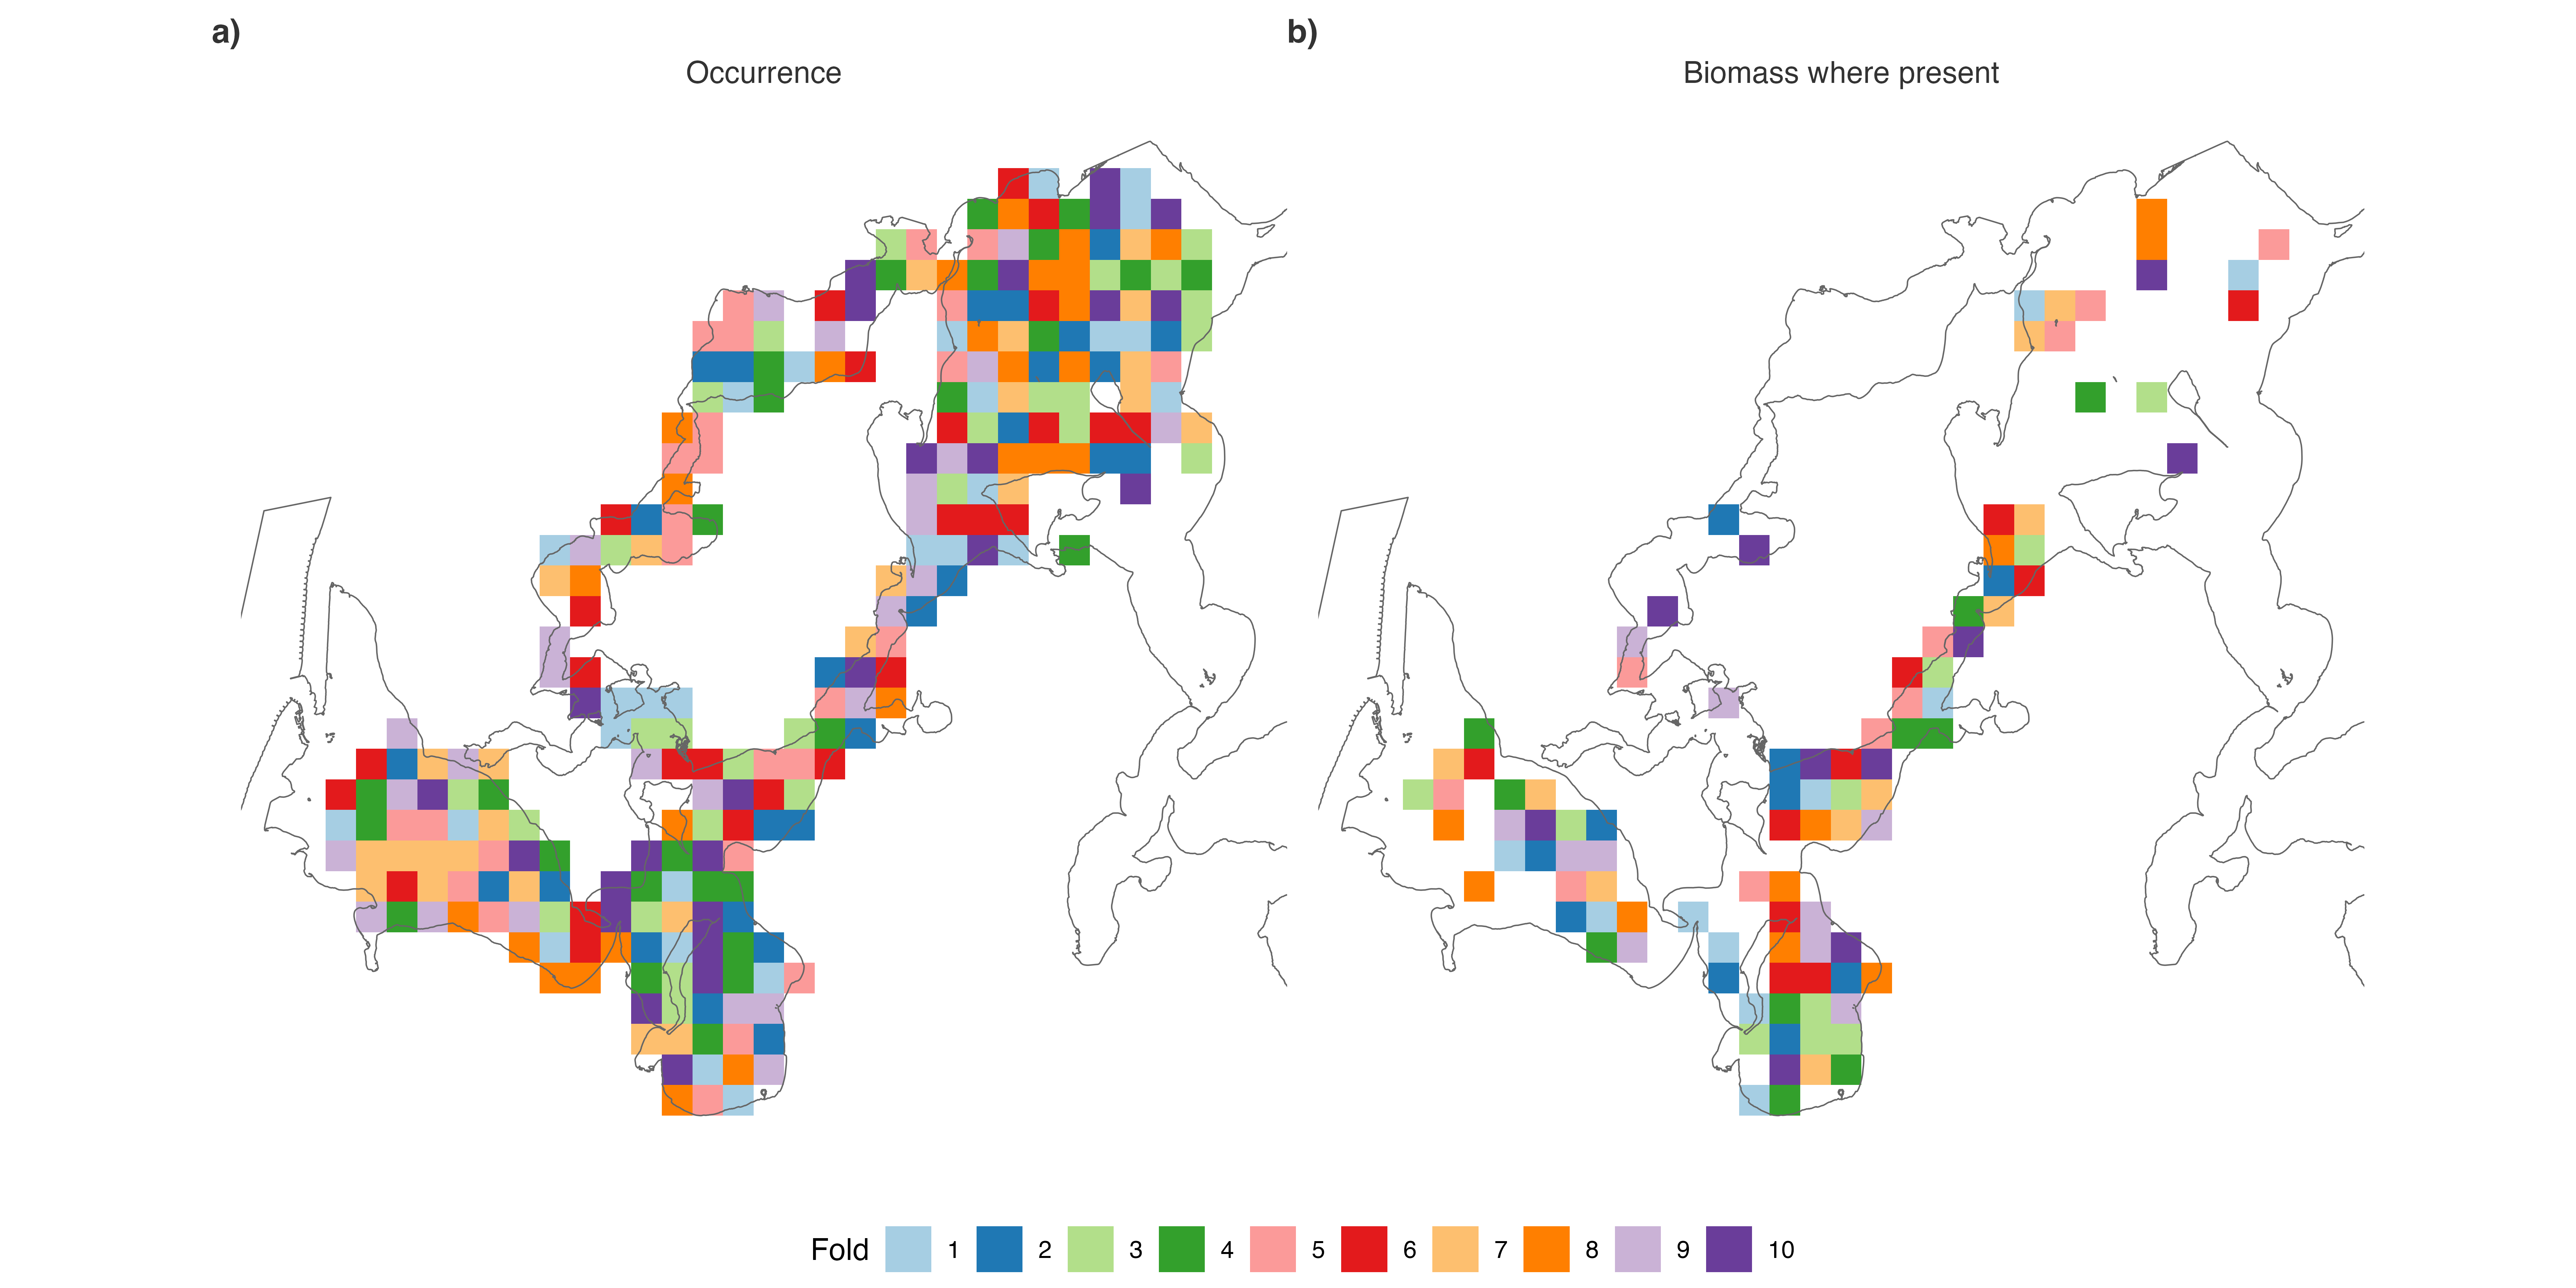
\includegraphics[width=0.95\textwidth]{figS5_cv_folds.png}
    \caption{Folds of the spatially blocked 10-fold cross-validation. Each 2~$\times$~2~km grid cell was a block, held out as a whole, and cells were randomly assigned to ten folds: (a) for the occurrence component, all cells containing survey stations; (b) for the positive-biomass component, the cells containing stations with cockles.}
    \label{fig:cv_folds}
\end{figure}
\clearpage

\begin{figure}[H]
    \centering
    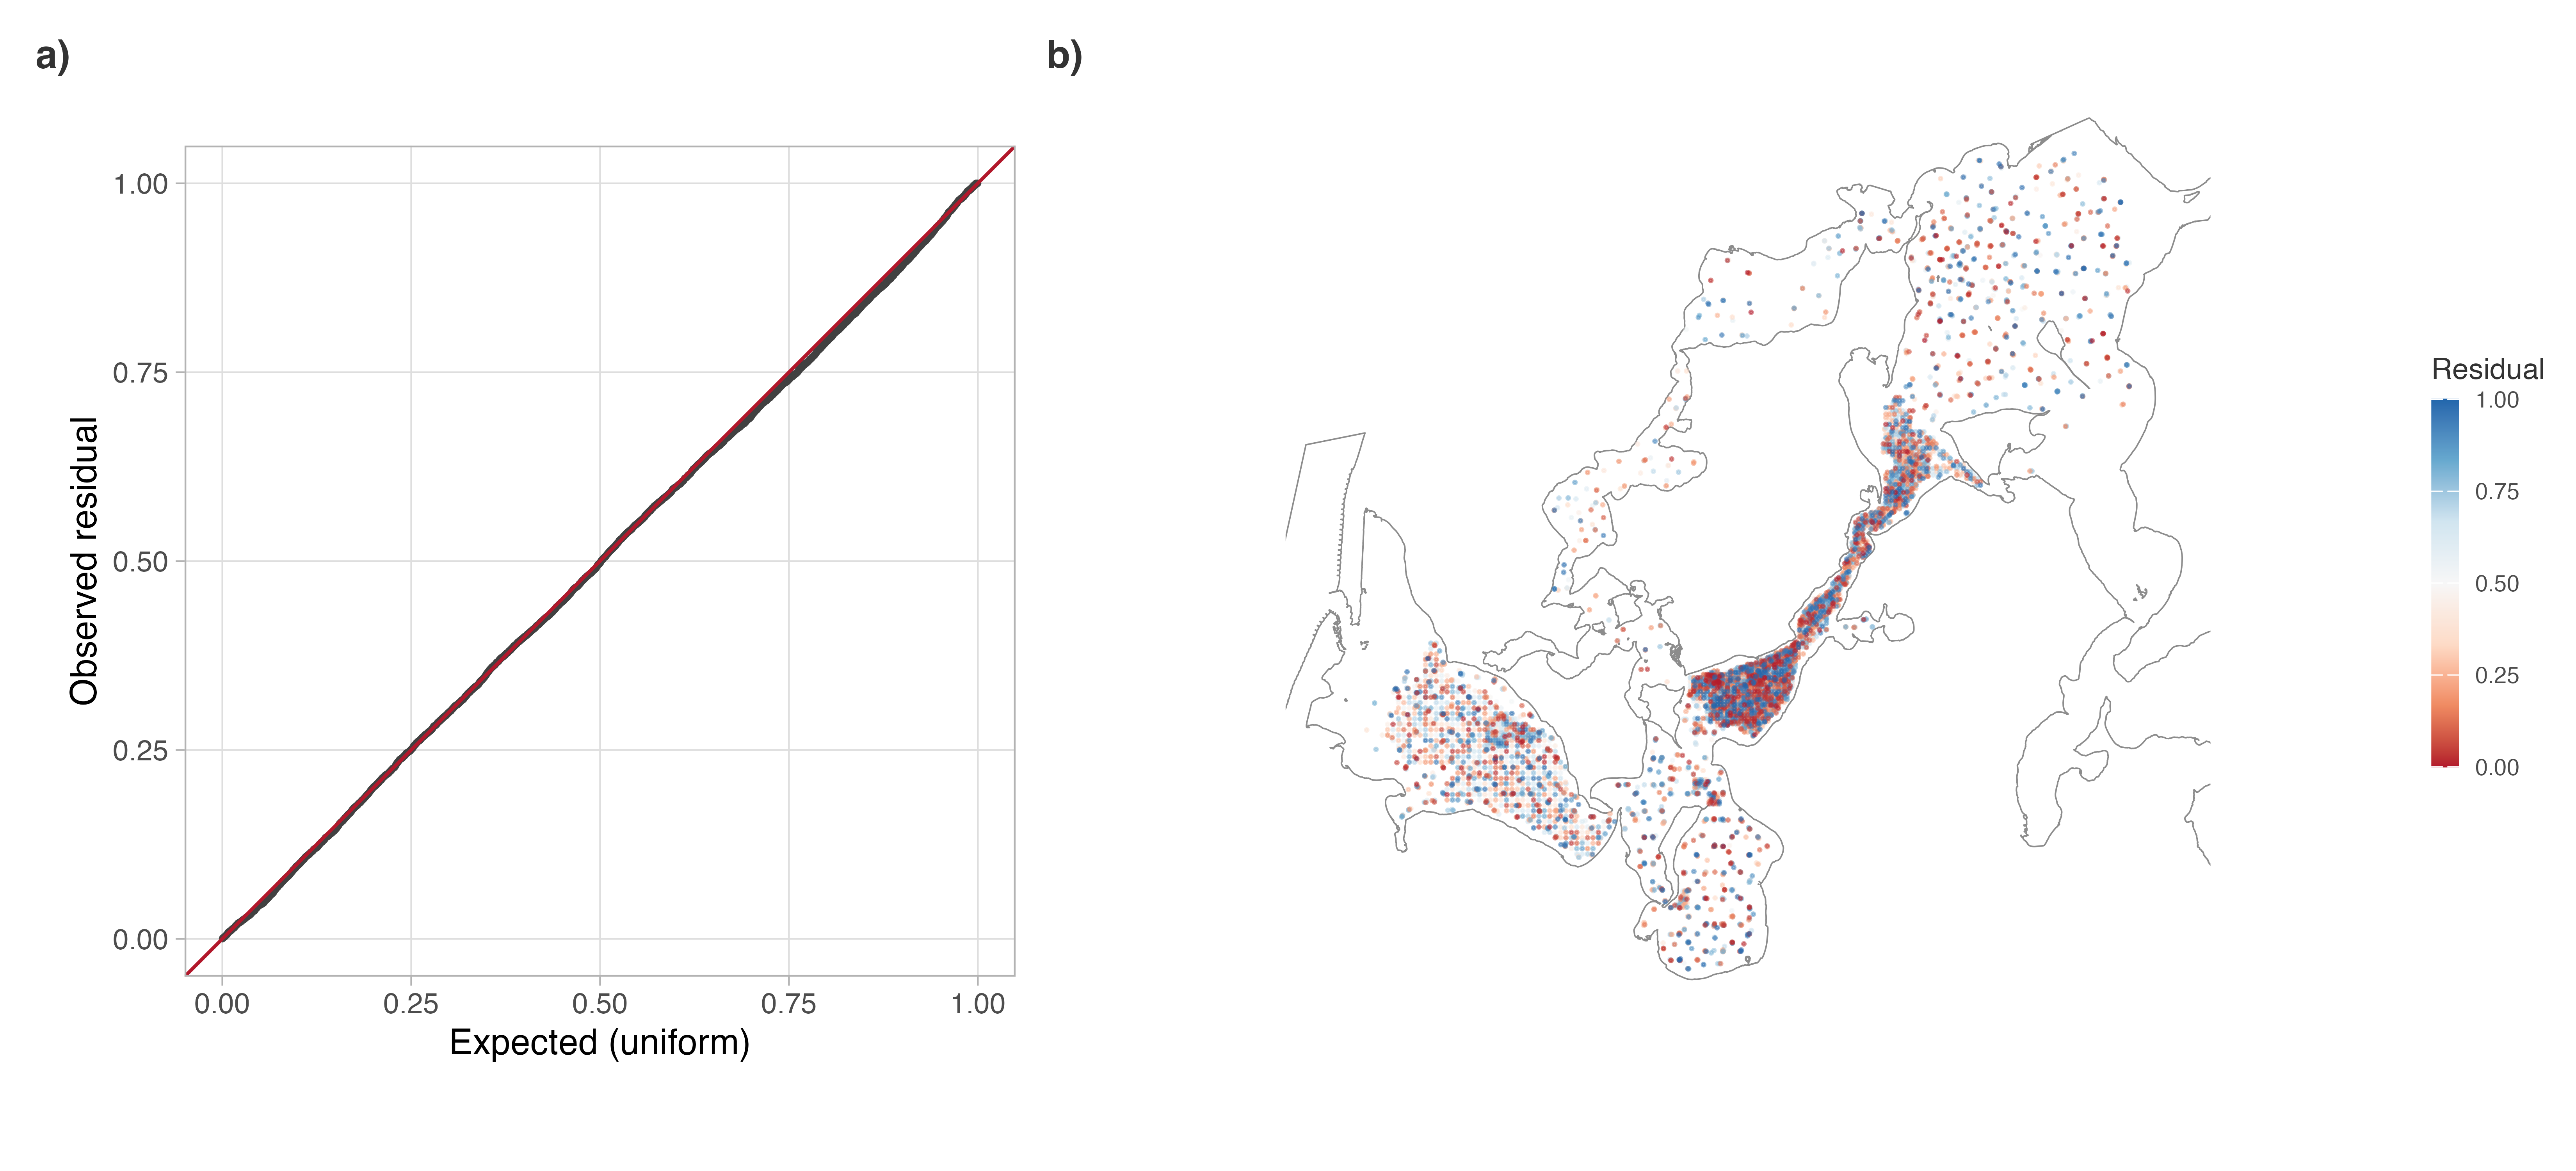
\includegraphics[width=0.95\textwidth]{figS6_residuals.png}
    \caption{Simulation-based residuals of the full Space + Environment + Connectivity model. For each station, 500 biomass values were simulated from the fitted delta-gamma model, drawing parameters from the multivariate normal distribution of the maximum-likelihood estimates, and the residual is the quantile of the observation among them (ties at zero randomised); residuals are uniform between 0 and 1 if the model is correct. (a) Q--Q plot against the uniform distribution (red line: 1:1); (b) residual at each station. The model reproduced the proportion of zeros (observed 0.812, simulated 0.798).}
    \label{fig:residuals}
\end{figure}
\clearpage

\begin{figure}[H]
    \centering
    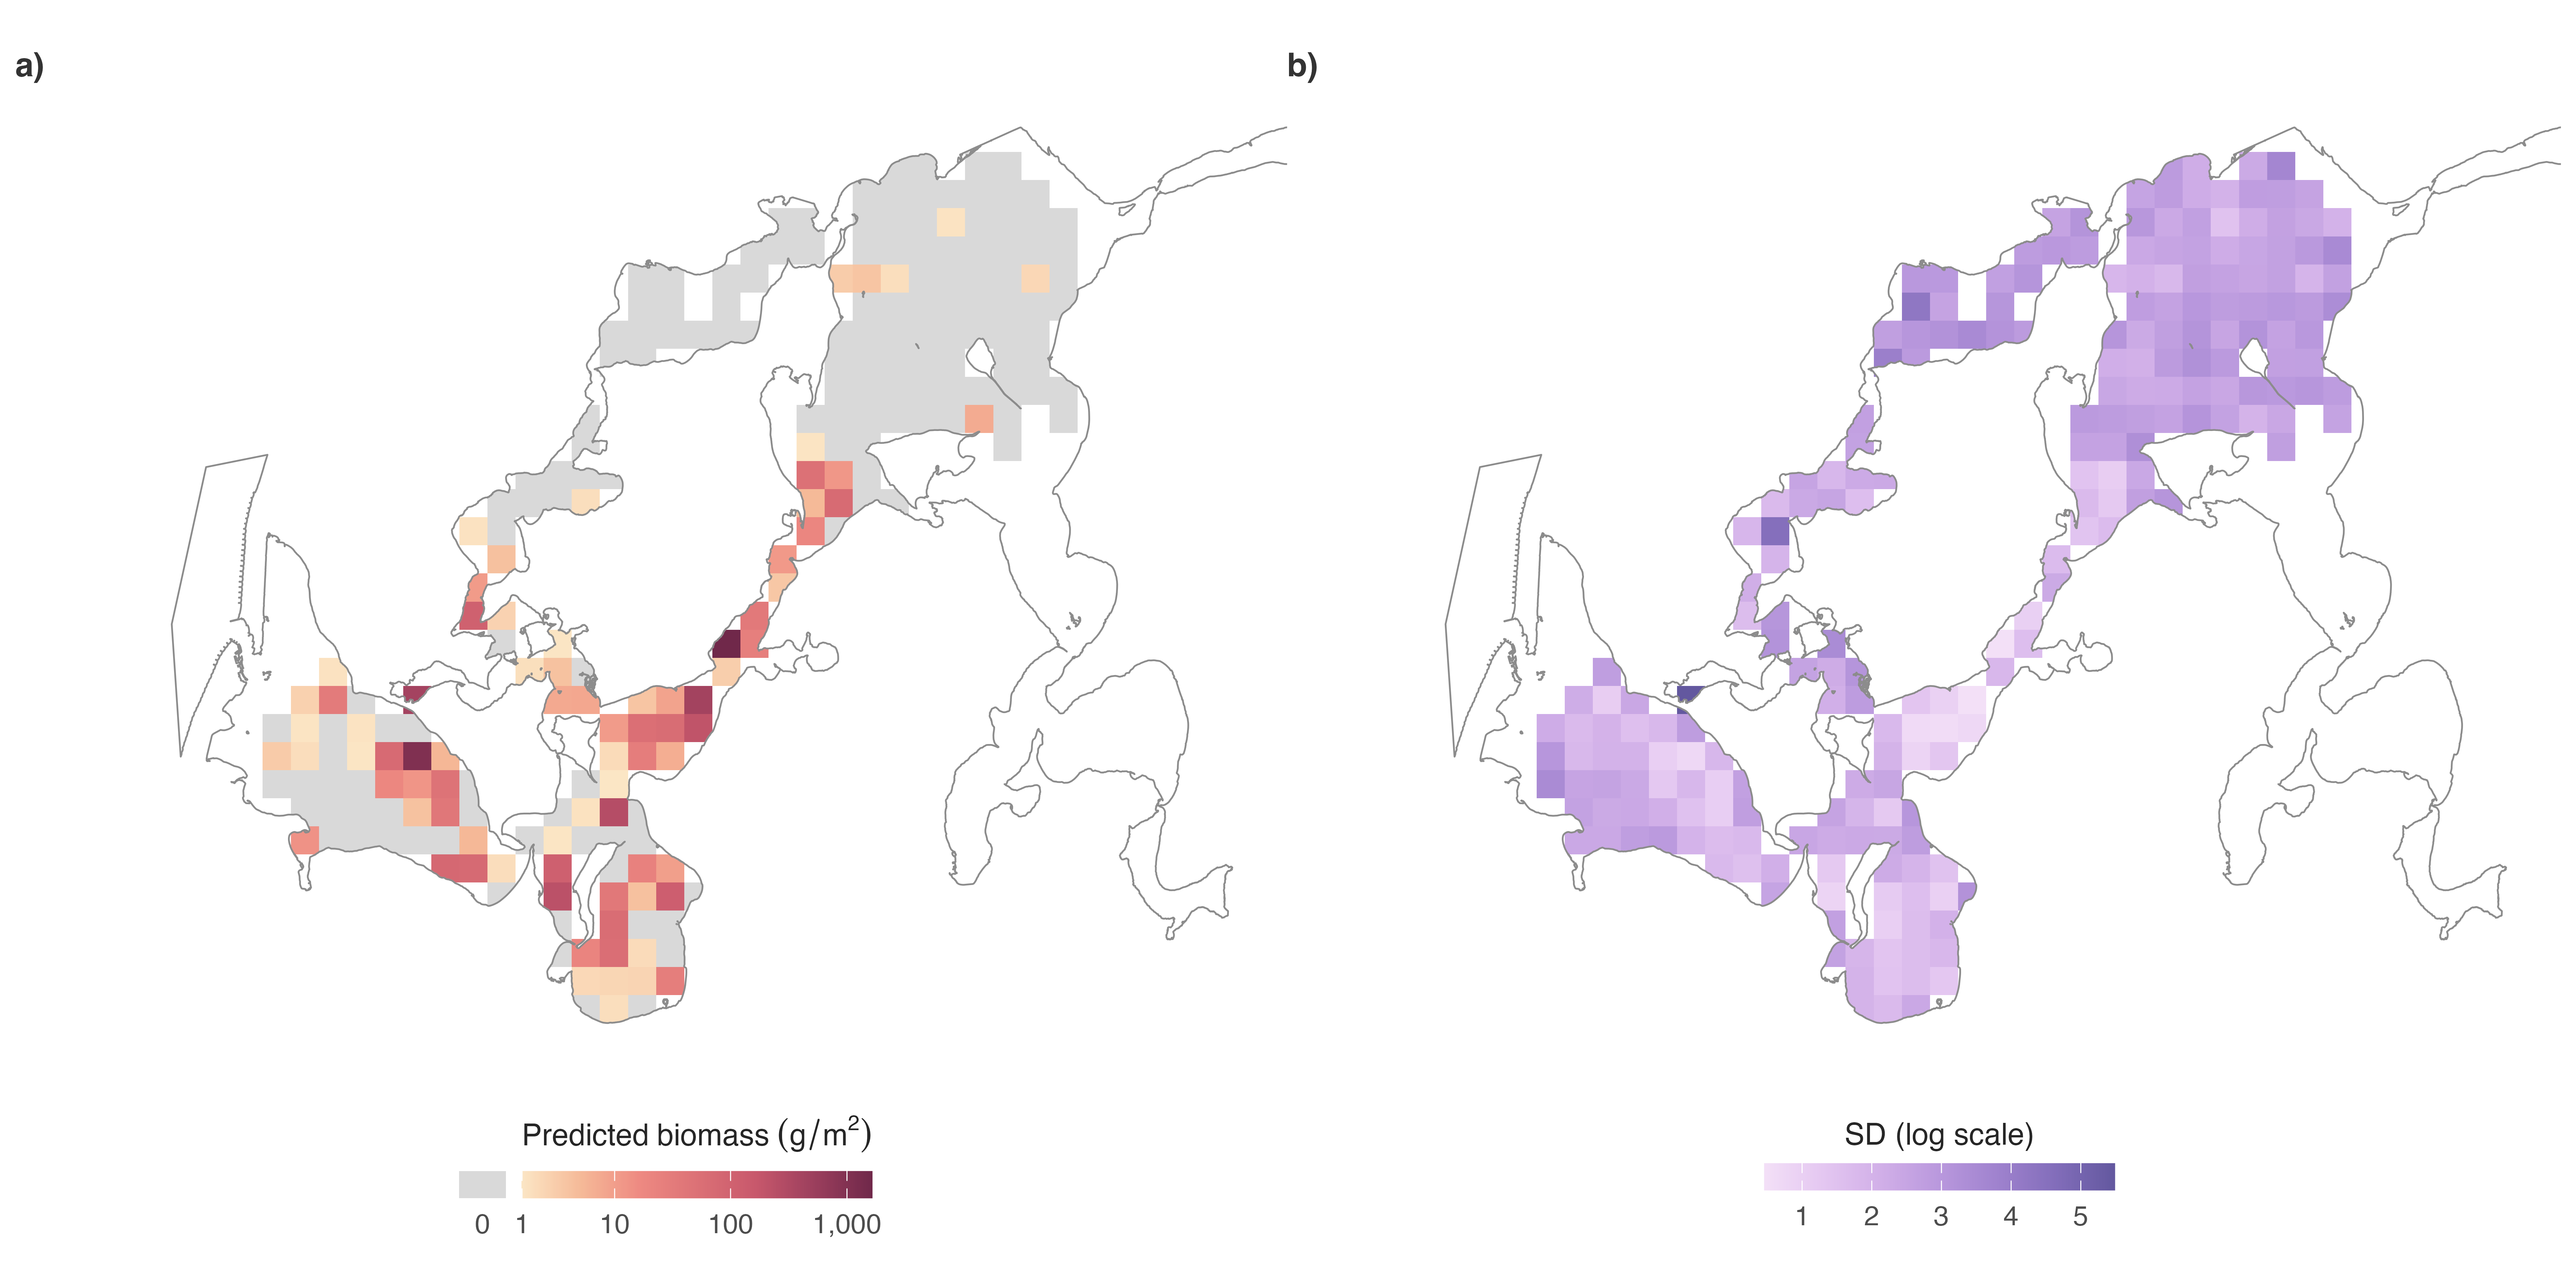
\includegraphics[width=0.95\textwidth]{figS7_predictions.png}
    \caption{(a) Cockle biomass density predicted by the full Space + Environment + Connectivity model at the centre of each 2~$\times$~2~km grid cell containing at least one survey station, for the 2021--2025 grab survey in 2025; grey cells have a predicted biomass below 1~g~m$^{-2}$. (b) Uncertainty of the prediction: standard deviation, on the log scale, of 500 draws from the joint precision matrix of the fitted model.}
    \label{fig:predictions}
\end{figure}
\clearpage

\begin{figure}[H]
    \centering
    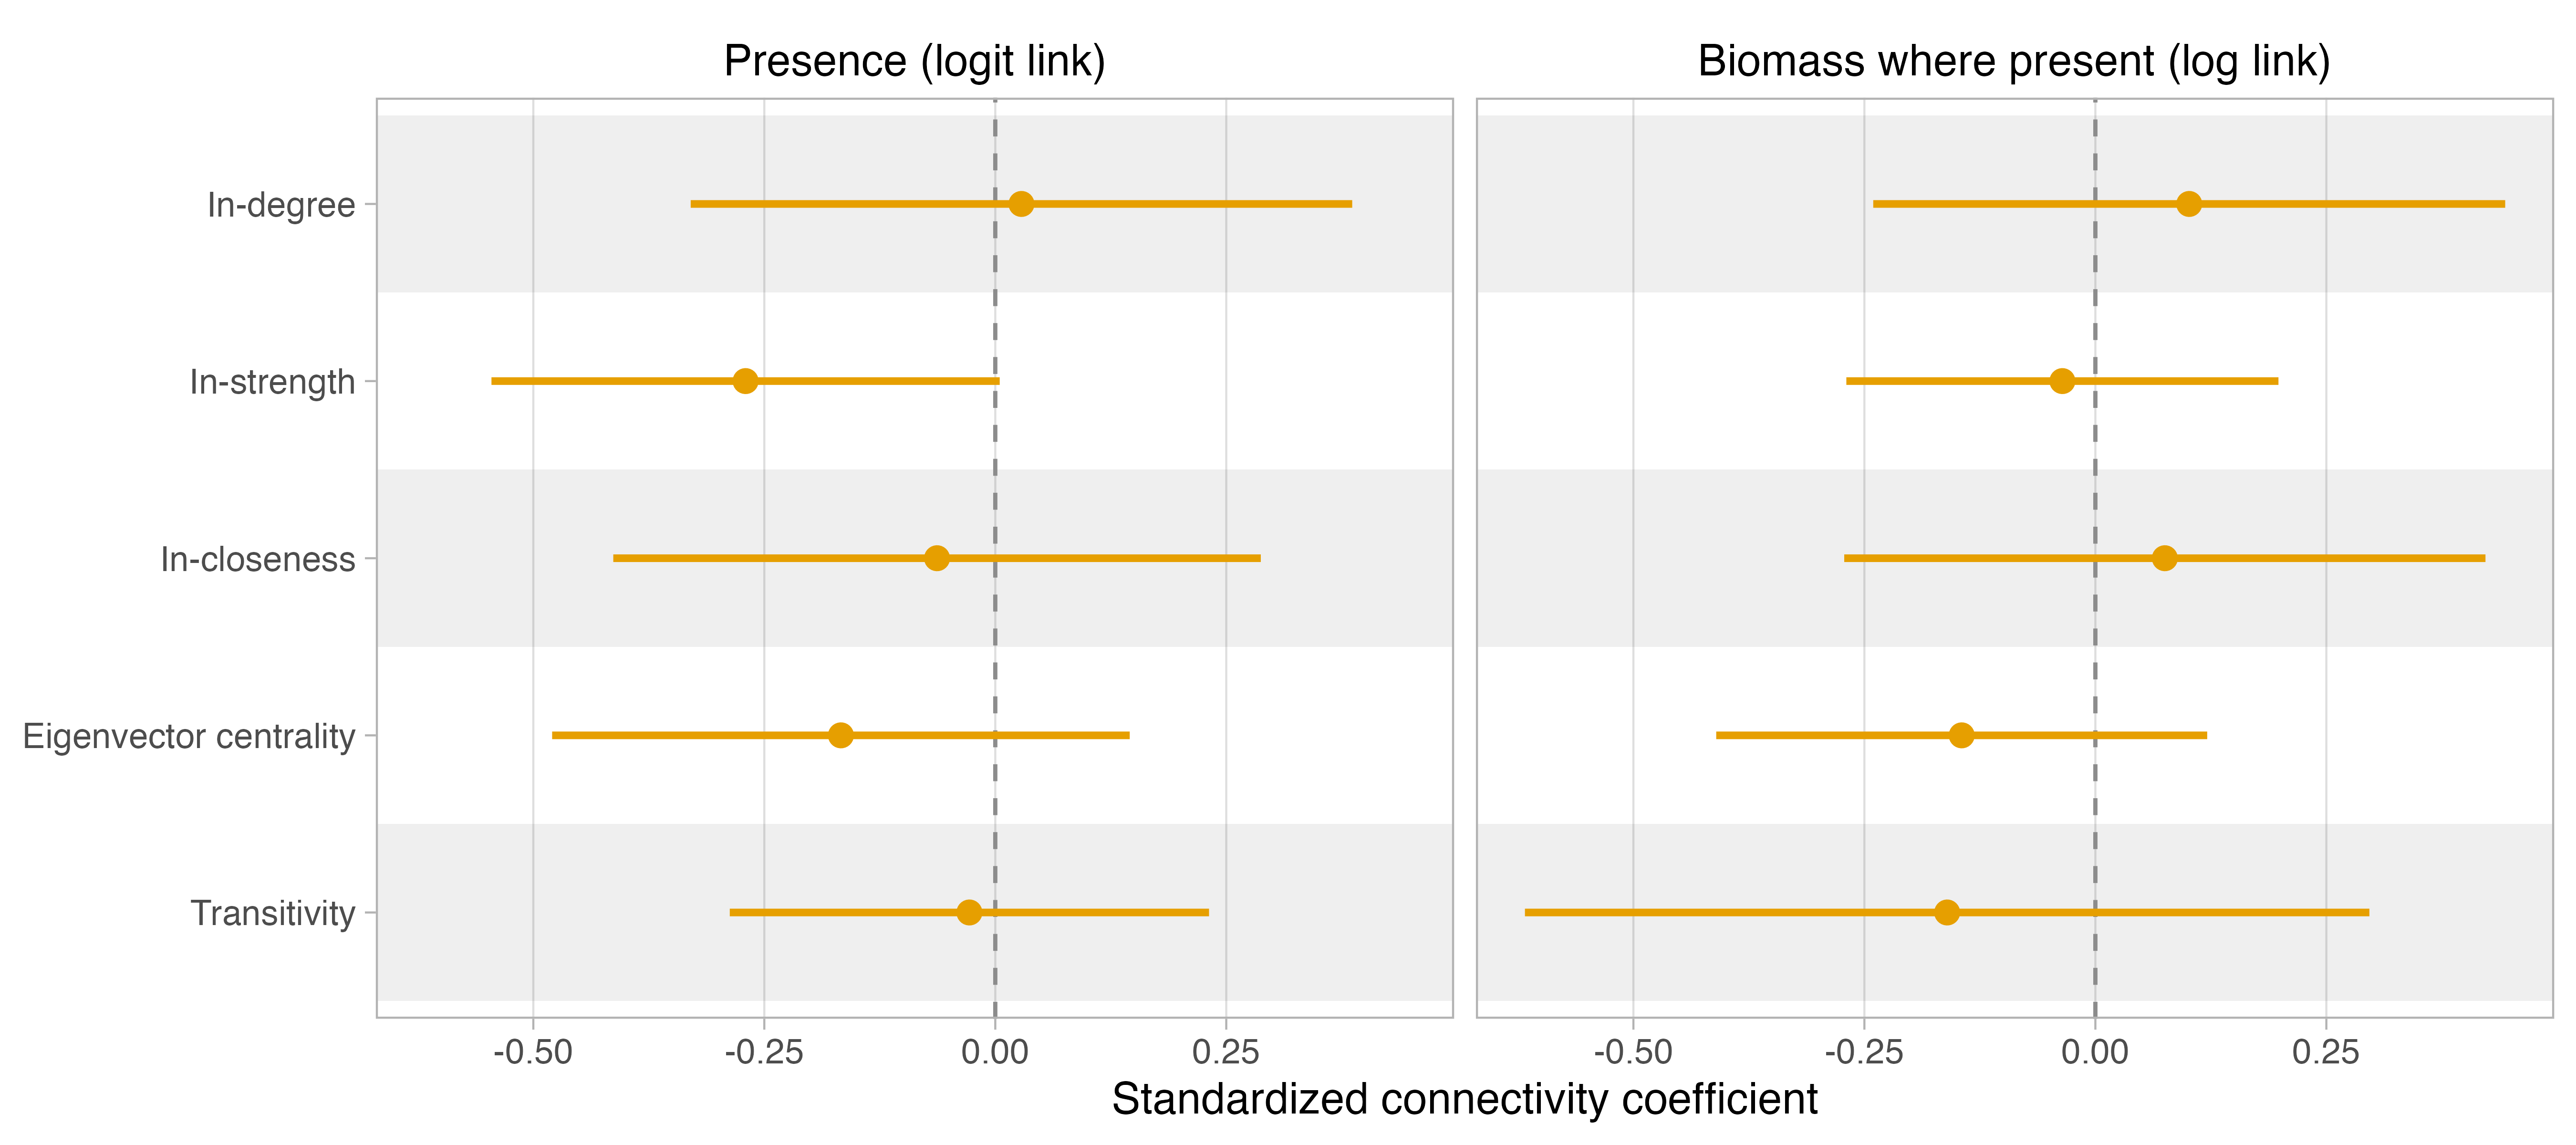
\includegraphics[width=0.95\textwidth]{figS8_connectivity_coefficients.png}
    \caption{Standardized connectivity coefficient, with 95\% confidence interval, in the full Space + Environment + Connectivity model fitted with each of the five connectivity metrics in turn, for the presence and biomass-where-present components.}
    \label{fig:connectivity_coefficients}
\end{figure}

\end{document}
